\documentclass[tikz,border=6pt]{standalone}
\usepackage{helvet}
\renewcommand{\familydefault}{\sfdefault}
\begin{document}
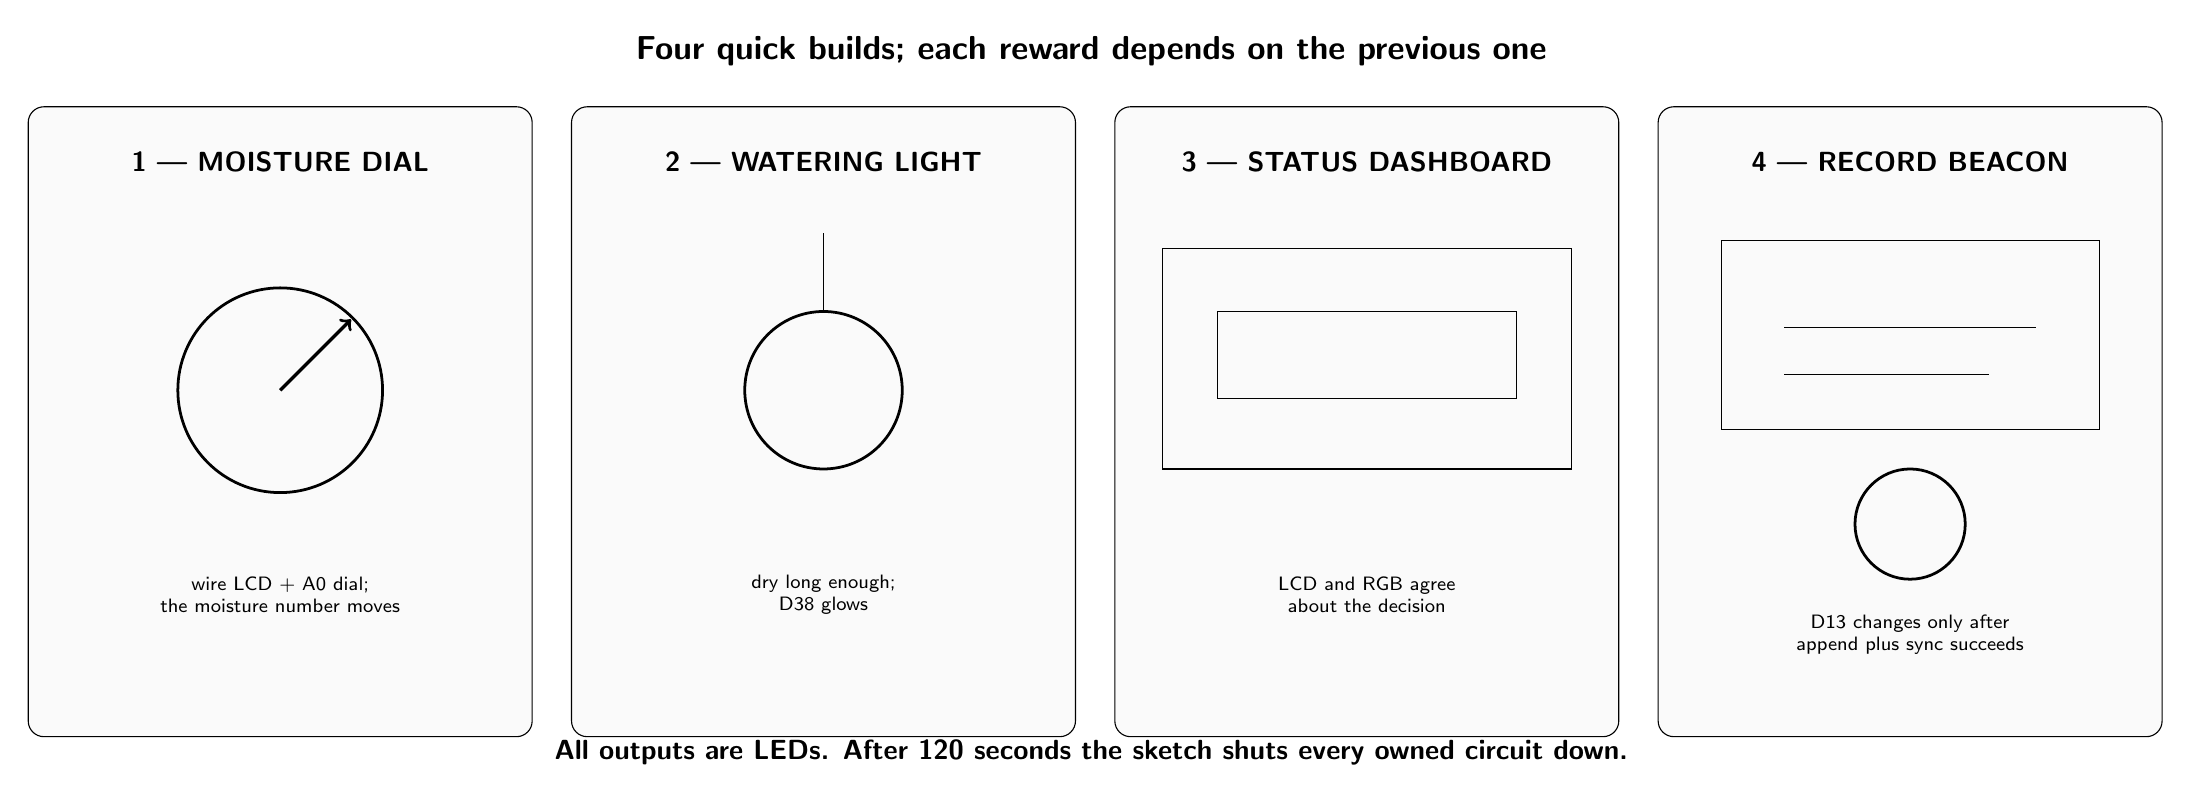
\begin{tikzpicture}[x=1mm,y=1mm,
  panel/.style={draw,rounded corners=2mm,fill=black!2,minimum width=64mm,minimum height=80mm},
  note/.style={font=\sffamily\scriptsize,align=center}]
\node[font=\sffamily\bfseries\large] at (138,91)
  {Four quick builds; each reward depends on the previous one};
\foreach \x/\n/\title in {35/1/MOISTURE DIAL,104/2/WATERING LIGHT,173/3/STATUS DASHBOARD,242/4/RECORD BEACON}
{
  \node[panel] at (\x,44) {};
  \node[font=\sffamily\bfseries] at (\x,77) {\n\ --- \title};
}
\draw[line width=1pt] (35,48) circle (13);\draw[->,line width=1.2pt] (35,48)--(44,57);
\node[note] at (35,22) {wire LCD + A0 dial;\\the moisture number moves};
\draw[line width=1pt] (104,48) circle (10);\draw (104,58)--(104,68);
\node[note] at (104,22) {dry long enough;\\D38 glows};
\draw (147,38) rectangle (199,66);\draw (154,47) rectangle (192,58);
\node[note] at (173,22) {LCD and RGB agree\\about the decision};
\draw (218,43) rectangle (266,67);\draw (226,56)--(258,56);\draw (226,50)--(252,50);
\draw[line width=1pt] (242,31) circle (7);
\node[note] at (242,17) {D13 changes only after\\append plus sync succeeds};
\node[note,font=\sffamily\bfseries] at (138,2)
  {All outputs are LEDs. After 120 seconds the sketch shuts every owned circuit down.};
\end{tikzpicture}
\end{document}
